\documentclass[border=8pt]{standalone}
\usepackage[T1]{fontenc}
\usepackage{tikz}
\usetikzlibrary{arrows.meta, positioning, decorations.pathreplacing, calc, fit}
\usepackage{amsmath}

% Color scheme
\definecolor{pipeblue}{RGB}{45,80,140}
\definecolor{pipefill}{RGB}{225,235,250}
\definecolor{refutegray}{RGB}{90,90,90}
\definecolor{loopred}{RGB}{160,50,50}
\definecolor{arrowgray}{RGB}{120,120,120}

\begin{document}
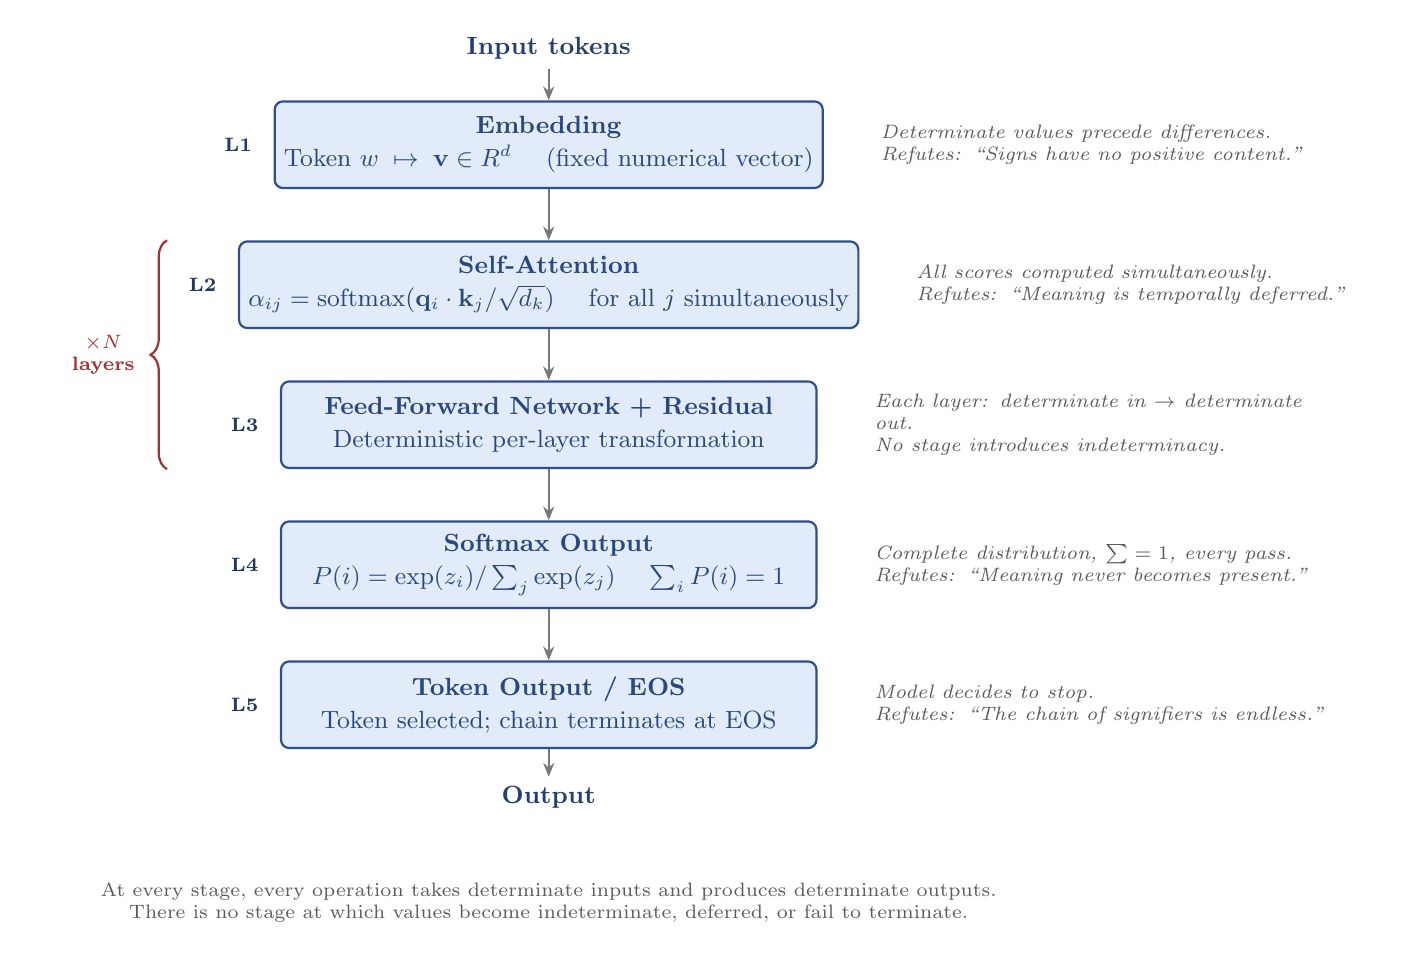
\begin{tikzpicture}[
    % Pipeline box style
    pipebox/.style={
        draw=pipeblue, fill=pipefill, thick,
        rounded corners=3pt,
        minimum width=6.8cm, minimum height=1.1cm,
        font=\small, align=center,
        text=pipeblue!90!black
    },
    % Refutation annotation style
    refute/.style={
        font=\scriptsize\itshape, align=left,
        text=refutegray, text width=5.8cm,
        anchor=west
    },
    % Arrow style
    pipelinearrow/.style={
        -{Stealth[length=5pt,width=4pt]},
        thick, color=arrowgray
    },
    % Level label style
    levellabel/.style={
        font=\scriptsize\bfseries, color=pipeblue!70!black
    }
]

% === PIPELINE BOXES ===

% Level 1
\node[pipebox] (L1) {%
    \textbf{Embedding}\\[1pt]
    Token $w \;\mapsto\; \mathbf{v} \in \mathbb{R}^d$ \quad (fixed numerical vector)
};

% Level 2
\node[pipebox, below=0.65cm of L1] (L2) {%
    \textbf{Self-Attention}\\[1pt]
    $\alpha_{ij} = \mathrm{softmax}(\mathbf{q}_i \cdot \mathbf{k}_j / \sqrt{d_k})$ \quad for all $j$ simultaneously
};

% Level 3
\node[pipebox, below=0.65cm of L2] (L3) {%
    \textbf{Feed-Forward Network + Residual}\\[1pt]
    Deterministic per-layer transformation
};

% Level 4
\node[pipebox, below=0.65cm of L3] (L4) {%
    \textbf{Softmax Output}\\[1pt]
    $P(i) = \exp(z_i) / \textstyle\sum_j \exp(z_j)$ \quad $\sum_i P(i) = 1$
};

% Level 5
\node[pipebox, below=0.65cm of L4] (L5) {%
    \textbf{Token Output / EOS}\\[1pt]
    Token selected; chain terminates at EOS
};

% === INPUT / OUTPUT LABELS ===
\node[above=0.4cm of L1, font=\small\bfseries, color=pipeblue!80!black] (input) {Input tokens};
\node[below=0.35cm of L5, font=\small\bfseries, color=pipeblue!80!black] (output) {Output};

% === ARROWS ===
\draw[pipelinearrow] (input) -- (L1);
\draw[pipelinearrow] (L1) -- (L2);
\draw[pipelinearrow] (L2) -- (L3);
\draw[pipelinearrow] (L3) -- (L4);
\draw[pipelinearrow] (L4) -- (L5);
\draw[pipelinearrow] (L5) -- (output);

% === LEVEL LABELS (left) ===
\node[levellabel, left=0.15cm of L1.west, anchor=east] {L1};
\node[levellabel, left=0.15cm of L2.west, anchor=east] {L2};
\node[levellabel, left=0.15cm of L3.west, anchor=east] {L3};
\node[levellabel, left=0.15cm of L4.west, anchor=east] {L4};
\node[levellabel, left=0.15cm of L5.west, anchor=east] {L5};

% === LOOP BRACE (L2--L3, N times) ===
% Use L2's x-coordinate for both endpoints to guarantee vertical brace
\draw[decorate, decoration={brace, amplitude=6pt, mirror}, thick, loopred]
    ([xshift=-0.9cm]L2.north west) -- ([xshift=-0.9cm]L2.north west |- L3.south west)
    node[midway, left=8pt, font=\scriptsize\bfseries, color=loopred, align=center]
    {$\times N$\\layers};

% === REFUTATION ANNOTATIONS (right) ===
\node[refute, right=0.6cm of L1.east] {%
    Determinate values precede differences.\\
    Refutes: ``Signs have no positive content.''
};
\node[refute, right=0.6cm of L2.east] {%
    All scores computed simultaneously.\\
    Refutes: ``Meaning is temporally deferred.''
};
\node[refute, right=0.6cm of L3.east] {%
    Each layer: determinate in $\to$ determinate out.\\
    No stage introduces indeterminacy.
};
\node[refute, right=0.6cm of L4.east] {%
    Complete distribution, $\sum = 1$, every pass.\\
    Refutes: ``Meaning never becomes present.''
};
\node[refute, right=0.6cm of L5.east] {%
    Model decides to stop.\\
    Refutes: ``The chain of signifiers is endless.''
};

% === BOTTOM SUMMARY LINE ===
\node[below=0.7cm of output, font=\scriptsize, text=refutegray, text width=13cm, align=center] {%
    At every stage, every operation takes determinate inputs and produces determinate outputs.\\
    There is no stage at which values become indeterminate, deferred, or fail to terminate.
};

\end{tikzpicture}
\end{document}
